%!TEX root=/home/ska124/Dropbox/Thesis/thes-full.tex

%%%%%%%%%%%%%%%%%%%%%%%%%%%%%%%%%%%%%%%%%%%%%%%%%
%
%     Chapter 5
%
%%%%%%%%%%%%%%%%%%%%%%%%%%%%%%%%%%%%%%%%%%%%%%%%

\chapter{Evaluation}
\label{chap:evaluation}
This chapter evaluates the performance of the \AC\ described in Chapter~\ref{chap:ac_architecture}. The evaluation is performed using the infrastructure described in Chapter~\ref{sec:simulation_infrastructure}. This chapter is divided into sections based on performance evaluations of:
\begin{itemize}[noitemsep]
	\item Comparison against a fixed granularity cache
	\item The spatial pattern predictor
	\item Adaptivity of the \AC\
	\item \AC\ versus other approaches
\end{itemize}

\section{Improved Memory Hierarchy Efficiency}
\label{sec:efficiency}
\vspace{5pt}
\noindent \textbf{Result 1:}{\emph~{\AC\ increases cache capacity by harvesting
  space from unused words and can achieve an 18\% reduction in both L1 and
  L2 miss rate.}
\\ \\
\noindent \textbf{Result 2:}{\emph~{\AC\ adaptively sizes the cache block
  granularity and reduces L1$\leftrightarrow$L2 bandwidth by 46\% and
  L2$\leftrightarrow$Memory bandwidth by 38\%.}
}
\\ \\
In this section, the bandwidth and miss rate properties of an \AC\ are compared against a conventional cache. A \textit{Fixed} cache represents a conventional cache which allocates a fixed granularity cache block on a refill request. The accuracy of the spatial pattern predictor is an important factor which governs the accuracy of the \AC\ and is evaluated separately. For the results presented in this section, cache line utilisation statistics, gathered from a prior run of the application on a conventional cache, are used to drive the predictor. This isolates the benefits of the \AC\ from the potentially changing accuracy of the spatial pattern predictor across different cache geometries. This also ensures that the spatial granularity predictions can be replayed across multiple simulation runs. To ensure equivalent data storage space, the \AC\ size is set to the sum of the tag array and the data array in a conventional cache. At the L1 level (64K), the net capacity of the \AC\ is 64K + 8*4*256 bytes and at the L2 level (1M) configuration, it is 1M + 8*8*2048 bytes. The L1 cache has 256 sets and the L2 cache has 2048 sets. 

Fig~\ref{fig:eval_scatter_bw_64k_1m} plots the miss rate and the traffic characteristics of the \AC{}.  Since \AC{} can hold blocks varying in size from 8B to 64B, each set can hold more blocks by utilizing the space saved from eliminating untouched words. The \AC\ reduces the 64K L1 miss rate on average by 23\%\footnote{All reported averages are geometric mean unless otherwise specified.} and standard deviation(SD) of 24 for the Low group, and by 21\%(SD:16) for the moderate group; even applications with high spatial locality experience a 7\%(SD:8) improvement in miss rate. There is a 46\%(SD:20) reduction on average in L1$\leftrightarrow$L2 bandwidth. At the 1M L2 level, the \AC\ improves the moderate group's miss rate by 8\%(SD:10) and bandwidth by 23\%(SD:12).  Applications with moderate utilization make better use of the space harvested from unused words by \AC{}. Many low utilization applications tend to be streaming and providing extra cache space does not help lower miss rate. However, by not fetching unused words, the \AC\ achieves a significant reduction (38\%(SD:24) on average) in off-chip L2$\leftrightarrow$Memory bandwidth; even High utilization applications see a 17\%(SD:15) reduction in bandwidth.  Utilization and miss rate are not, however, always directly correlated (more details in \S~\ref{sec:adaptivity}).

With the \AC\, the number of blocks per set varies based on the granularity of the blocks being fetched, which in turn depends on the spatial locality in the application. Table~\ref{table:blockcount} shows the average number of blocks per set. In applications with low spatial locality, the \AC\ adjusts the block size and adapts to store many smaller blocks. The 64K L1 \AC\ stores 10 blocks per set for mcf and 12 blocks per set for art, effectively increasing associativity without introducing hardware overheads. At the L2, when the working set starts to fit in the L2 cache, the set is partitioned into fewer blocks. 

\begin{figure}[ht]

  \subfloat[64K - Low]{
    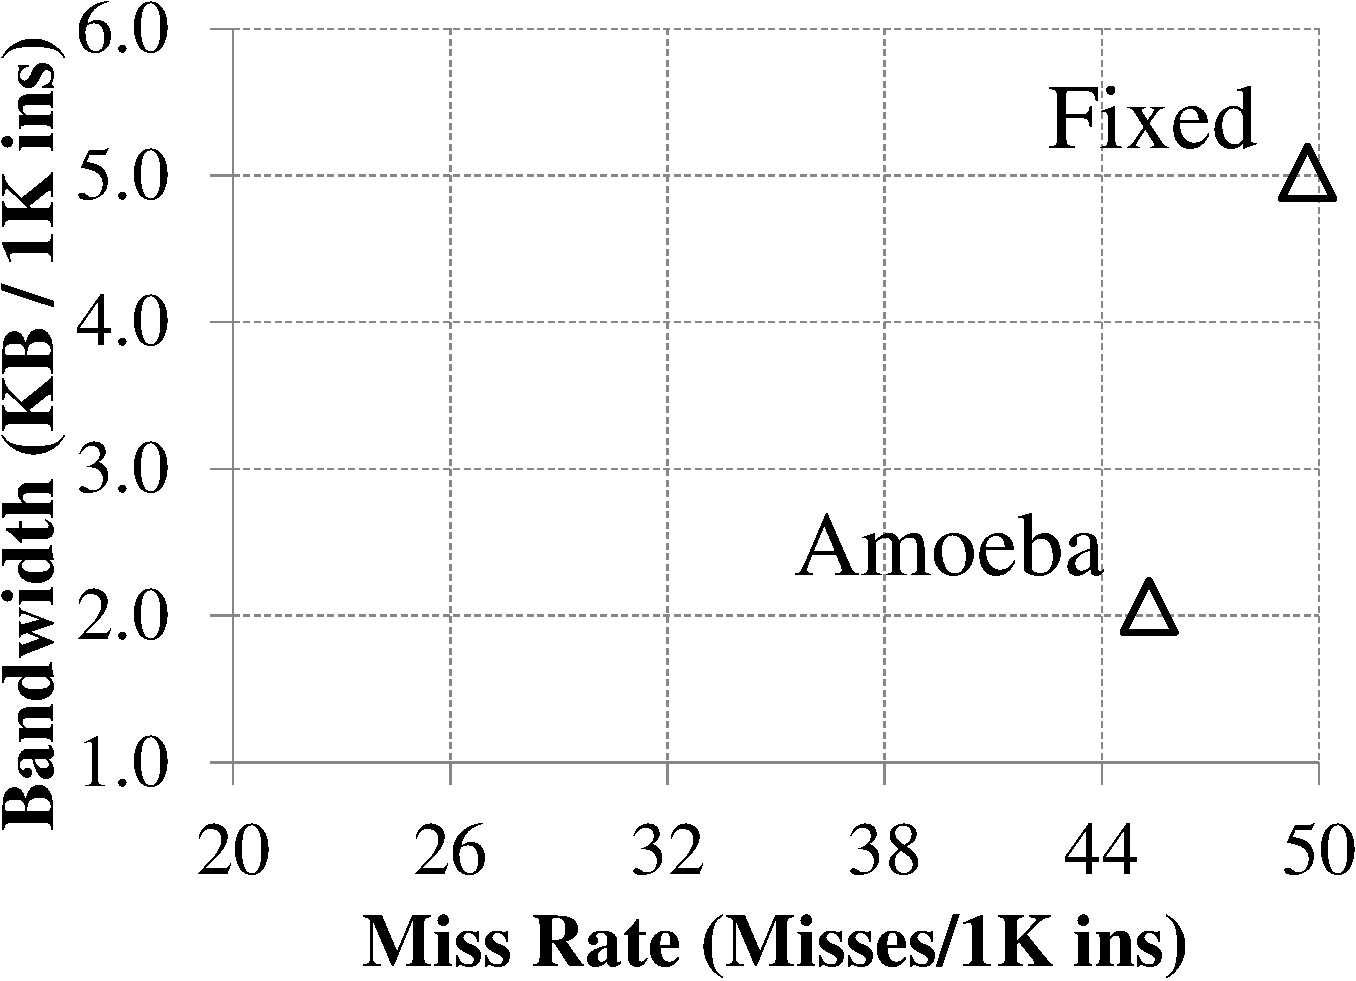
\includegraphics[width=0.48\textwidth]{files/Plots/08-Scatter_Bw_Miss_64K_low.pdf}
  }
  \subfloat[1M - Low]{
     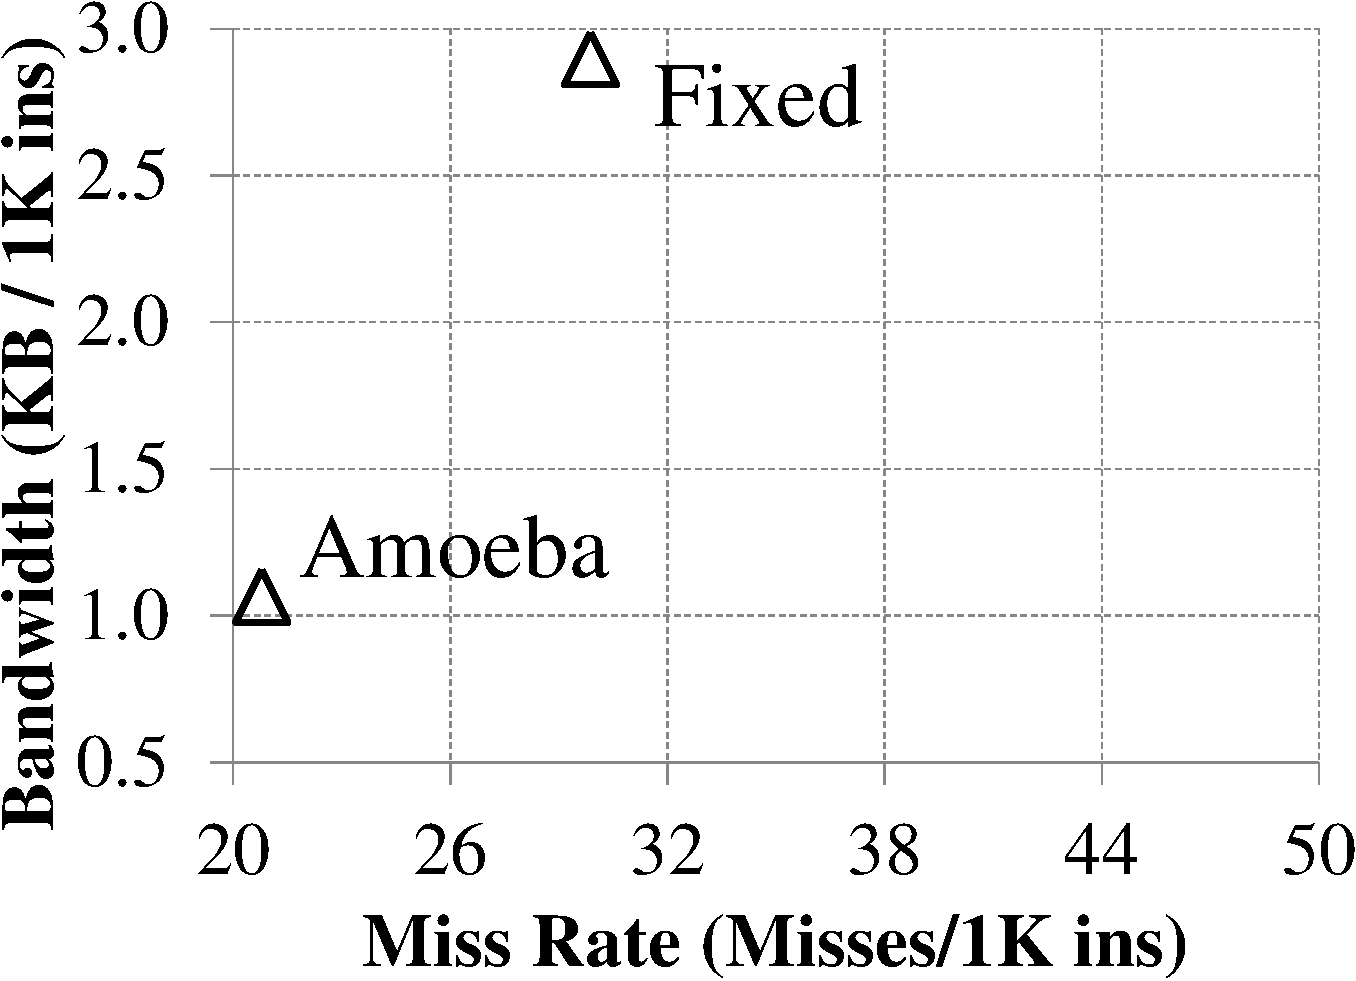
\includegraphics[width=0.48\textwidth]{files/Plots/08-Scatter_Bw_Miss_1M_low.pdf}
  }
  
  \subfloat[64K - Moderate]{
    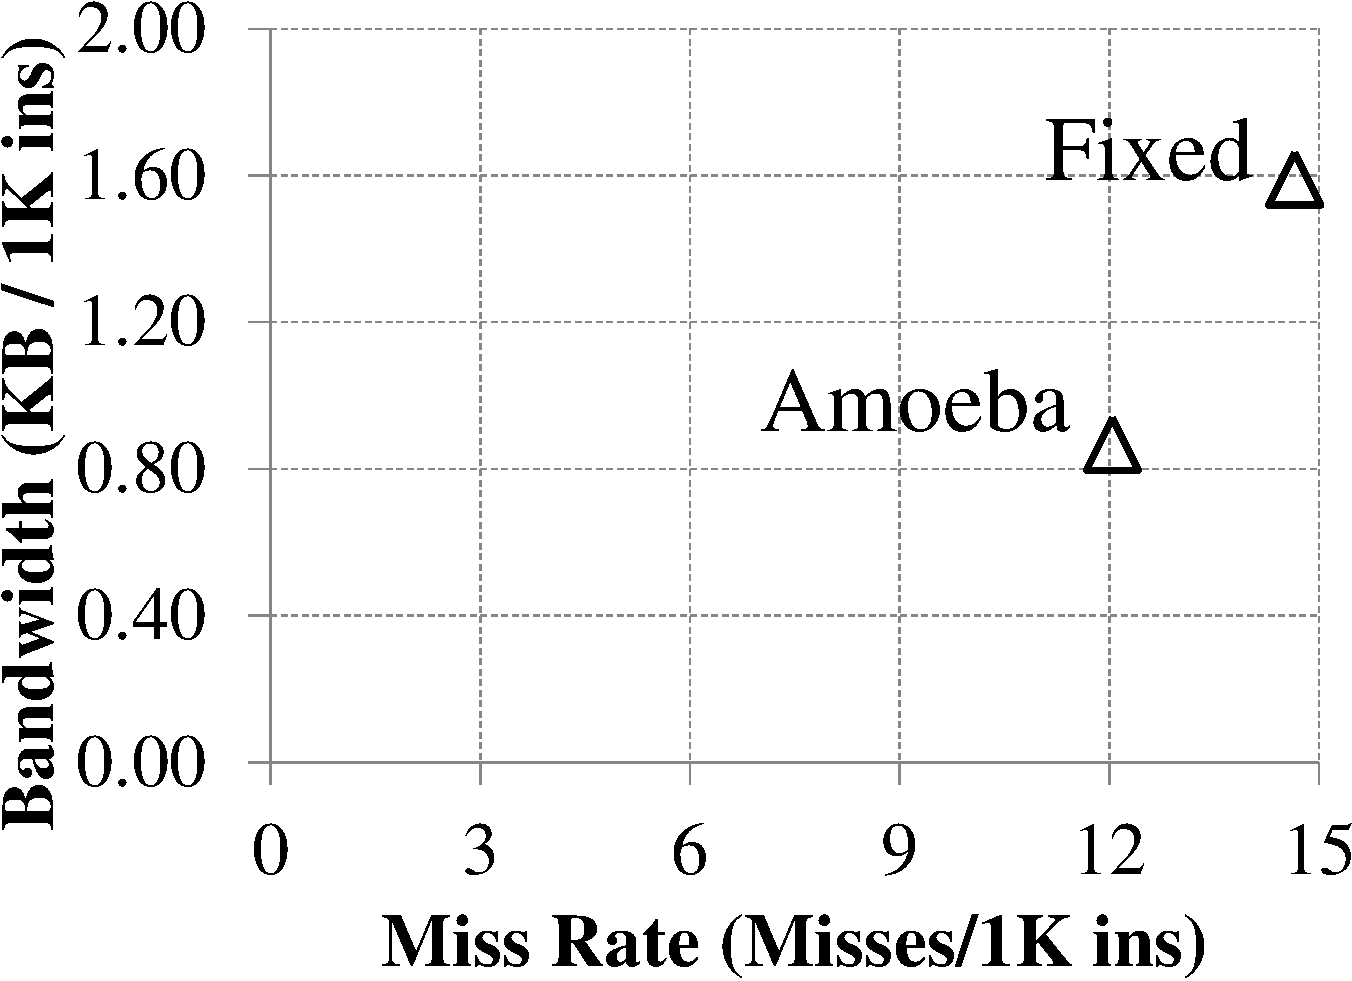
\includegraphics[width=0.48\textwidth]{files/Plots/08-Scatter_Bw_Miss_64K_mod.pdf}
  }
  \subfloat[1M - Moderate]{
     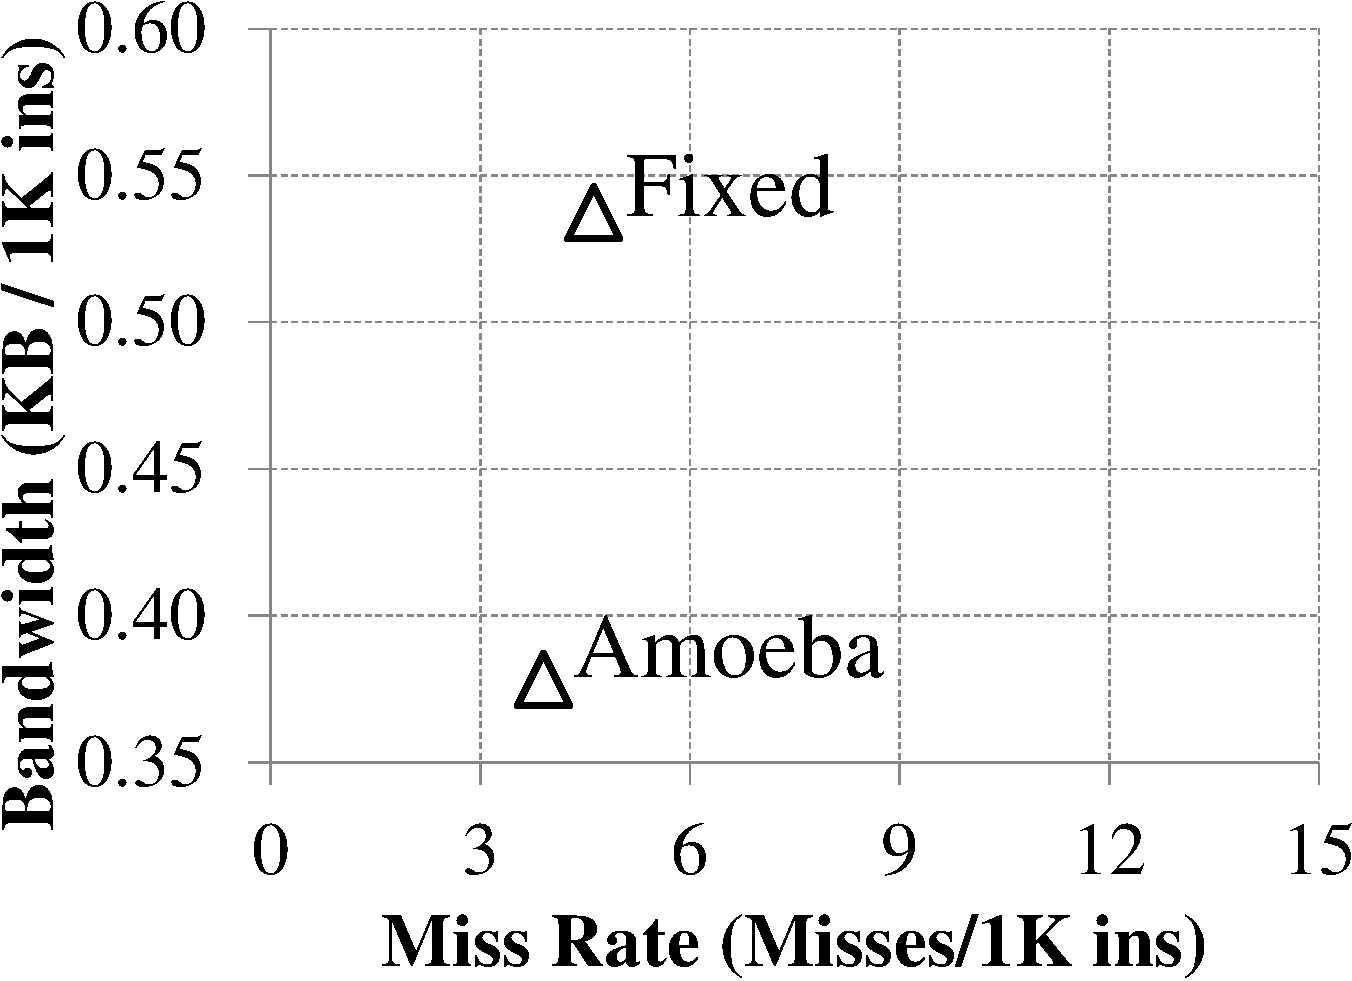
\includegraphics[width=0.48\textwidth]{files/Plots/08-Scatter_Bw_Miss_1M_mod.pdf}
  }
    
  \subfloat[64K - High]{
    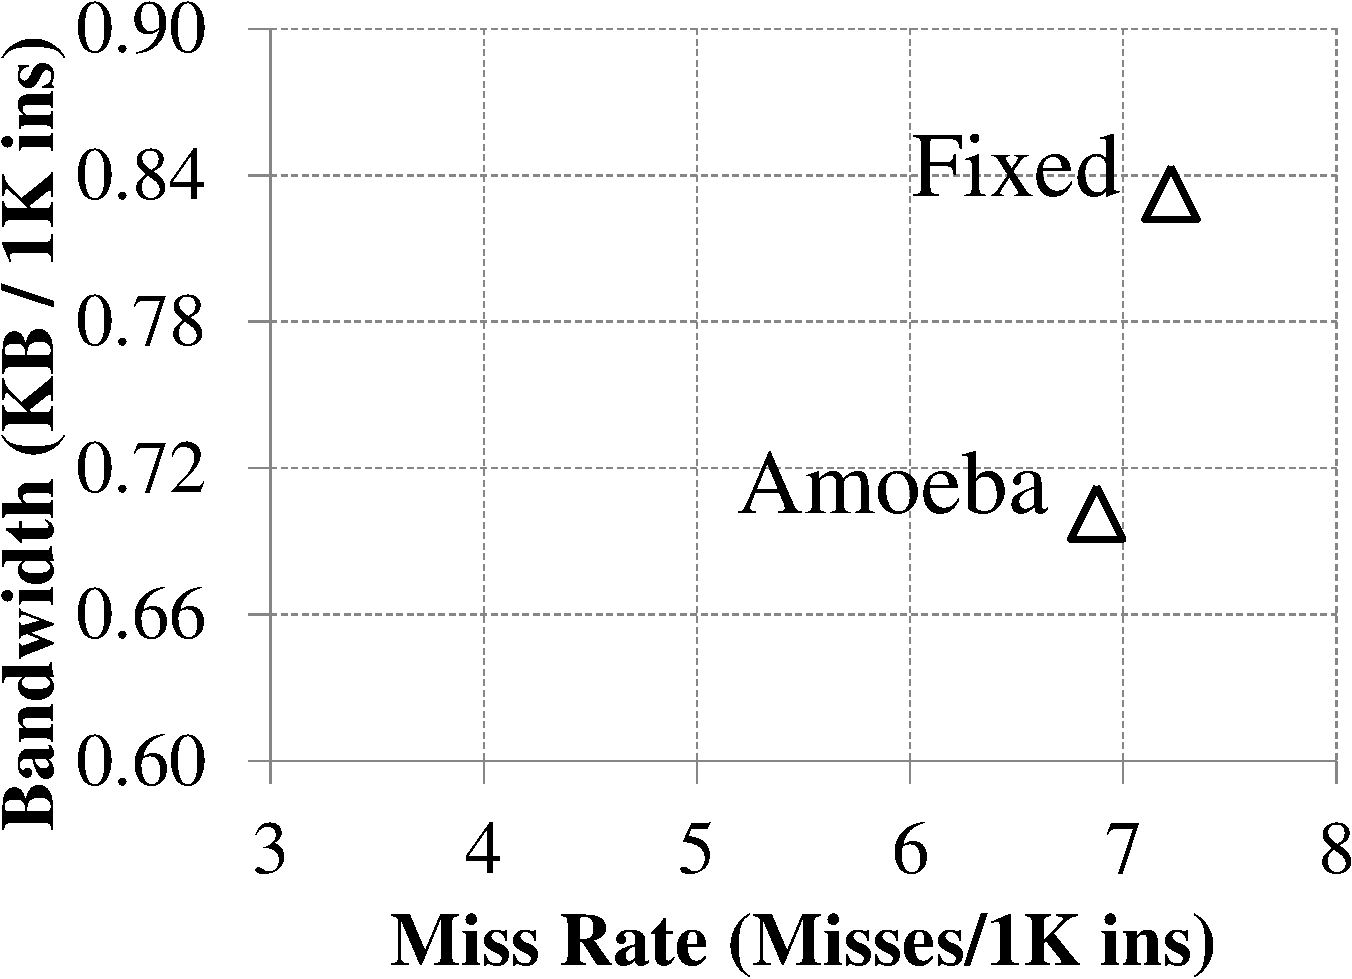
\includegraphics[width=0.48\textwidth]{files/Plots/08-Scatter_Bw_Miss_64K_high.pdf}
  }
  \subfloat[1M - High]{
     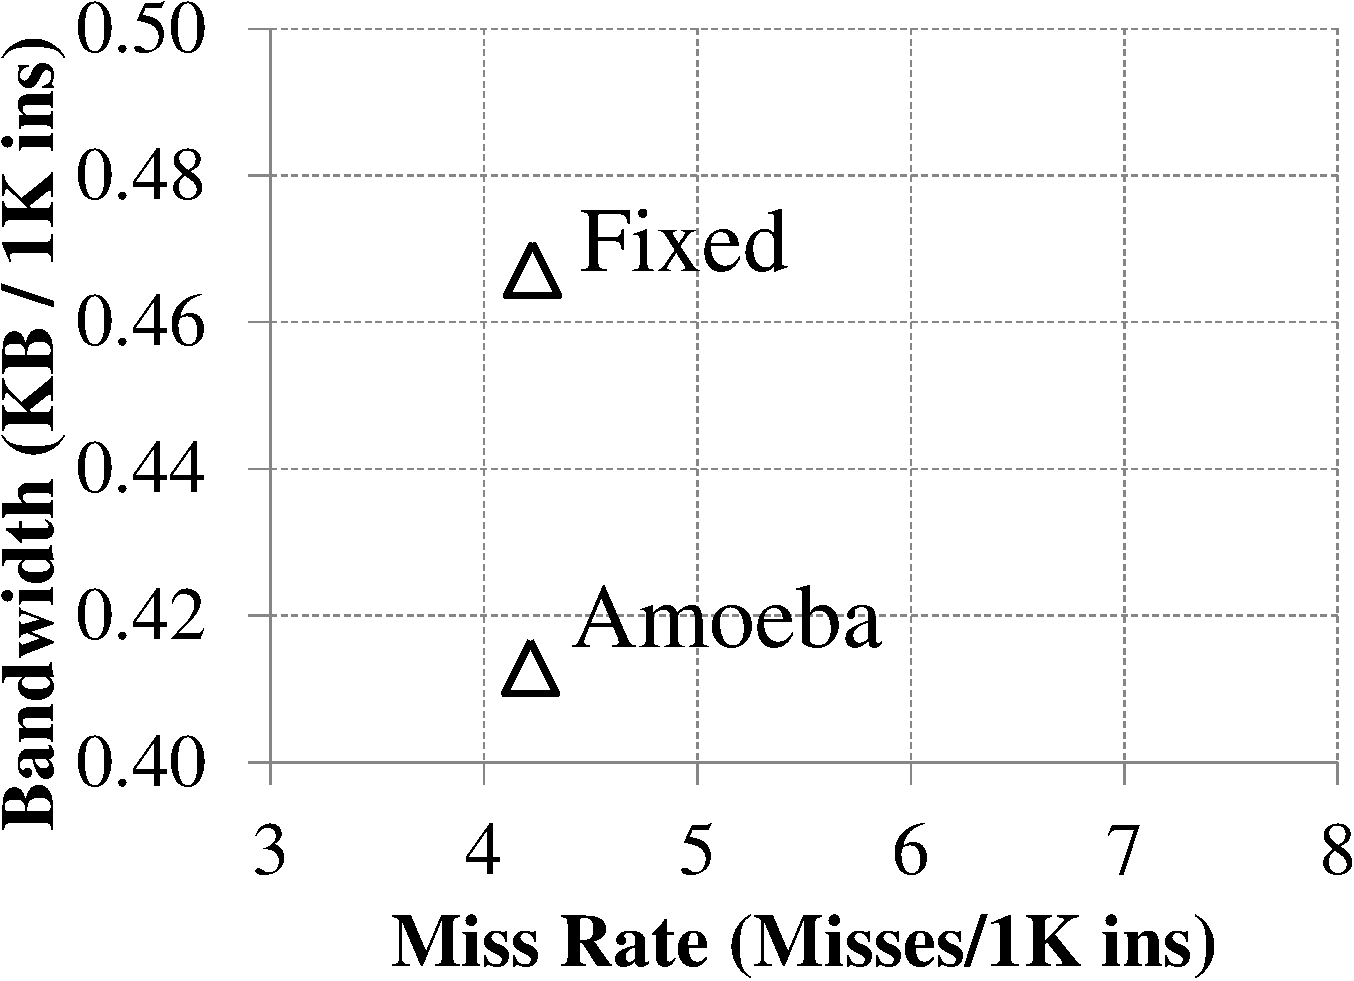
\includegraphics[width=0.48\textwidth]{files/Plots/08-Scatter_Bw_Miss_1M_high.pdf}
  }

  \caption[Bandwidth vs. Miss Rate]{Bandwidth vs. Miss Rate for a fixed granularity cache and \AC{}. (a),(c),(e): 64K, 4-wayL1 equivalent (b),(d),(f): 1M, 8-way LLC equivalent.  Markers on the plot indicate cache block size. Note the different scales for different groups.}
  \label{fig:eval_scatter_bw_64k_1m}
\end{figure}

\clearpage

%!TEX root=/home/ska124/Dropbox/Thesis/thes-full.tex
\begin{table}[h]
  \centering
  \begin{tabular}{|c|c|}
  \hline 
    Blocks/Set & 64K Cache, 288 B/set \\
    \hline
    4---5  &  ferret, cactus, firefox, eclipse, facesim, freqmine, milc, astar\\
    6---7  &  tpc-c, tradesoap, soplex, apache, fluidanimate\\
    8---9  &  h2, canneal, omnetpp, twolf, x264, lbm, jbb \\
    10---12 & mcf, art \\
    \hline
    \multicolumn{2}{c}{} \\
    \hline
    Blocks/Set & 1M Cache, 576 B/set \\
    \hline
    3---5 & eclipse, omnetpp   \\
    8---9 & cactus, firefox, tradesoap, freqmine, h2, x264, tpc-c   \\
    10---11  & facesim, soplex, astar, milc, apache, ferret  \\
    12---13  & twolf, art, jbb, lbm , fluidanimate \\
    15---18 & canneal, mcf \\
    \hline
  \end{tabular}
  \caption[Amoeba Blocks per set]{Average number of \AB{}s per set}
  \label{table:blockcount}
\end{table}


\begin{figure}[!h]
  \centering
  \subfloat[64K L1 cache]{
    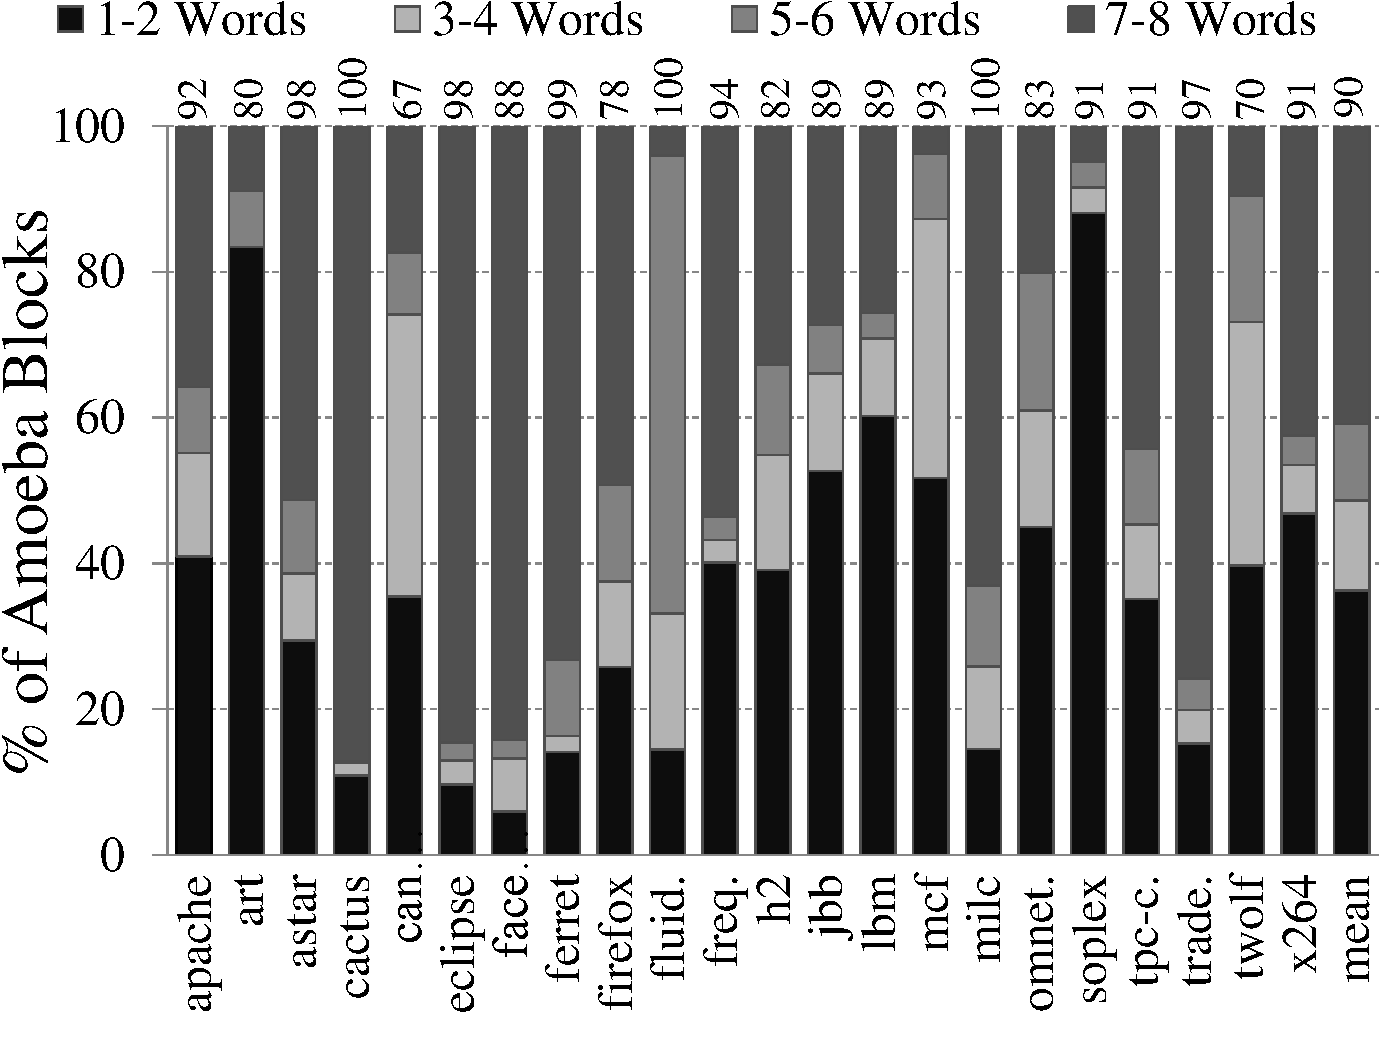
\includegraphics[width=0.8\textwidth]{files/Plots/08-StackBar_PredictSize_64K.pdf}
  }

  \subfloat[1M L2 cache]{
    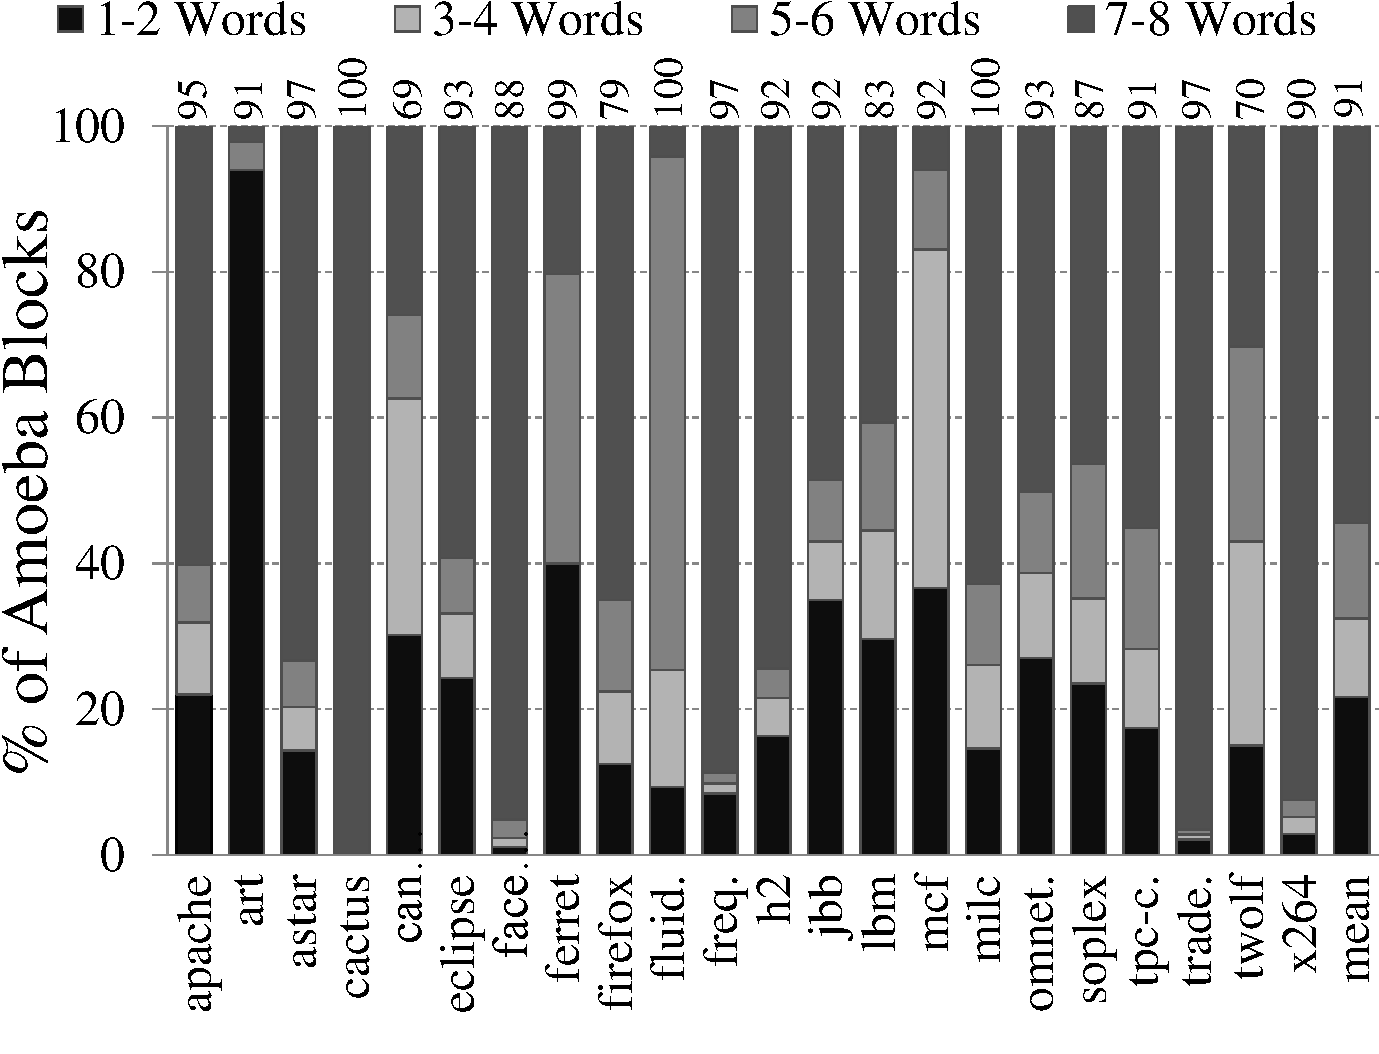
\includegraphics[width=0.8\textwidth]{files/Plots/08-StackBar_PredictSize_1M.pdf}
  }
  \caption[Distribution of cache block sizes]{Distribution of cache line granularities in the (a) 64K L1 and (b) 1M L2 \AC{}. Average utilization is on top.}
  \label{fig:StackBar_PredictorSize_64K}
\end{figure}

Note that applications like eclipse and omnetpp hold only 3---5 blocks per set on average (lower than conventional associativity) due to their low miss rates (see Table~\ref{table:Abs_Eval_Oracle}). With streaming applications (e.g., canneal), \AC\ increases the number of blocks/set to $>$15 on average. Finally, some applications like apache store between 6---7 blocks/set with a 64K cache with varied block sizes (see Figure~\ref{fig:StackBar_PredictorSize_64K}): approximately 50\% of the blocks store 1-2 words and 30\% of the blocks store 8 words at the L1. As the size of the cache increases and thereby the lifetime of the blocks, the \AC\ adapts to store larger size blocks as can be seen in Figure~\ref{fig:StackBar_PredictorSize_64K}.

Utilization is improved greatly across all applications (90\%+ in many cases). Figure~\ref{fig:StackBar_PredictorSize_64K} shows the distribution of cache block granularities in \AC{}. The \AB\ distribution matches the word access distribution presented in Fig~\ref{fig:stackbar_words_64k}). With the 1M cache, the larger cache size improves block lifespan and thereby utilization, with a significant drop in the \% of 1---2 word blocks. However, in many applications (tpc-c, apache, firefox, twolf, lbm, mcf), up to 20\% of the blocks are 3--6 words wide, indicating the benefits of adaptivity and the challenges faced by a fixed granularity conventional cache.

%!TEX root=/home/ska124/Dropbox/Thesis/thes-full.tex
\begin{table}[h]
\centering
	\begin{tabular}{|c|c|c|c|c|c|c|c|c|}
	\hline
	 & \multicolumn{2}{c|}{MPKI} &  \multicolumn{2}{c|}{BW Bytes/1K} & CPI & \multicolumn{2}{c|}{Predictor Stats}  \\
	\hline
	          & L1        & L2    & L1$\longleftrightarrow$L2 & L2$\longleftrightarrow$Mem & & FT &  \\
	          & MPKI & MPKI & Bytes/1K & Bytes/1K & Cycles/Ins. & Miss \% &  Ins/Evict\\
	\hline
	apache    &    64.9 & 19.6    &    5,000  &    2,067         &  8.3  & 0.4 &   17 \\
	art       &    133.7  &    53.0    &    5,475  &    1,425    &  16.0 & 0.0 &   9 \\
	astar     &    0.9    &    0.3     &    70     &    35       &  1.9  & 18.0 &  1,600 \\
	cactus    &    6.9    &    4.4     &    604    &    456      &  3.5  & 7.5 &   162 \\
	canne.    &    8.3    &    5.0     &    486    &    357      &  3.2  & 5.8 &   128 \\
	eclip.    &    3.6    &    $<$0.1  &    433    &    $<$1     &  1.8  & 0.1 &   198 \\
	faces.    &    5.5    &    4.7     &    683    &    632      &  3.0  & 41.2 &  190 \\
	ferre.    &    6.8    &    1.4     &    827    &    83       &  2.1  & 1.3 &   156 \\
	firef.    &    1.5    &    1.0     &    123    &    95       &  2.1  & 11.1 &  727 \\
	fluid.    &    1.7    &    1.4     &    138    &    127      &  1.9  & 39.2 &  629 \\
	freqm.    &    1.1    &    0.6     &    89     &    65       &  2.3  & 17.7 &  994 \\
	h2        &    4.6    &    0.4     &    328    &    46       &  1.8  & 1.7 &   154 \\
	jbb       &    24.6   &    9.6     &    1,542  &    830      &  5.0  & 10.2 &  42 \\
	lbm       &    63.1   &    42.2    &    3,755  &    3,438    &  13.6 & 6.7 &   18 \\
	mcf       &    55.8   &    40.7    &    2,519  &    2,073    &  13.2 & 0.0 &   19 \\
	milc      &    16.1   &    16.0    &    1,486  &    1,476    &  6.0  & 2.4 &   66 \\
	omnet.    &    2.5    &    $<$0.1  &    158    &    $<$1     &  1.9  & 0.0 &   458 \\
	sople.    &    30.7   &    4.0     &    1,045  &    292      &  3.1  & 0.9 &   35 \\
	tpcc      &    5.4    &    0.5     &    438    &    36       &  2.0  & 0.4 &   200 \\
	trade.    &    3.6    &    $<$0.1  &    410    &    6        &  1.8  & 0.6 &   194 \\
	twolf     &    23.3   &    0.6     &    1,326  &    45       &  2.2  & 0.0 &   49 \\
	x264      &    4.1    &    1.8     &    270    &    190      &  2.2  & 12.4 &  274 \\
	\hline                                  
	\end{tabular}                                                                       
                                                                       
\caption[Absolute performance statistics]{Abslute performance statistics for the \AC\ using a \code{Region} predictor(infinite table size) with predictions for compulsory misses serviced using data collected from a prior run of the application. Higher value for Ins/Evict indicates predictor training takes longer. \\ \\
	\textbf{MPKI} : Misses / 1K instructions. \\
	\textbf{BW}: Number of words / 1K instructions. \\
	\textbf{CPI}: Clock cycles per instruction. \\
	\textbf{FT}: Percentage of misses that are compulsory misses.  \\
	\textbf{Ins/Evict}: Number of instructions between evictions. 
}
\label{table:Abs_Eval_Oracle}                                        
\end{table}                                                          
\clearpage

% First Touch info for Inf Table
% 0.4
% 0.0
% 18.0
% 7.5
% 5.8
% 0.1
% 41.2
% 1.3
% 11.1
% 39.2
% 17.7
% 1.7
% 10.2
% 6.7
% 0.0
% 2.4
% 0.0
% 0.9
% 0.4
% 0.6
% 0.0
% 12.4

% First Touch info for 1K Table
% 16.0
% 0.0
% 20.1
% 9.5
% 44.0
% 0.1
% 76.3
% 20.1
% 44.9
% 86.6
% 19.3
% 2.7
% 55.4
% 57.0
% 13.6
% 93.2
% 0.0
% 1.9
% 5.1
% 0.6
% 0.0
% 19.0


% Instructions per Eviction data for Oracle 64K

% 17
% 9
% 1,600
% 162
% 128
% 198
% 190
% 156
% 727
% 629
% 994
% 154
% 42
% 18
% 19
% 66
% 458
% 35
% 200
% 194
% 49
% 274

\section{Overall Performance and Energy}

\noindent \textbf{Result 3:}{~\AC\ improves overall cache efficiency and boosts performance by 10\% on commercial applications\footnote{``Commercial'' applications includes Apache, SpecJBB and TPC-C.}, saving up to 11\% of the energy of the on-chip memory hierarchy. Off-chip L2$\leftrightarrow$memory energy sees a mean reduction of 41\% across all workloads (86\% for art and 93\% for twolf). 
\\ \\
A two-level cache hierarchy is modeled in which the L1 is a 64K cache with 256 sets (3 cycles load-to-use) and the L2 is 1M, 8192 sets (20 cycles). A fixed memory latency of 300 cycles is assumed. It is assumed that the L1 access is the critical pipeline stage and throttle CPU clock by 4\% (an alternative approach is evaluated in the next section).  The total dynamic energy of the \AC\ is calculated using the energy numbers determined in Section~\ref{sec:area_latency_energy_overhead} through a combination of synthesis and CACTI~\cite{Muralimanohar:2007:ONO:1331699.1331704}. 4 fast tags per set at the L1 and 8 fast tags per set at the L2 are used. The penalty for all the extra metadata in the \AC{} is included. The energy for a single L1---L2 transfer (6.8pJ per byte) is derived from~\cite{weti,Muralimanohar:2007:ONO:1331699.1331704}. The interconnect uses full-swing wires at 32nm, 0.6V. 

\begin{figure}[h]
  \centering
    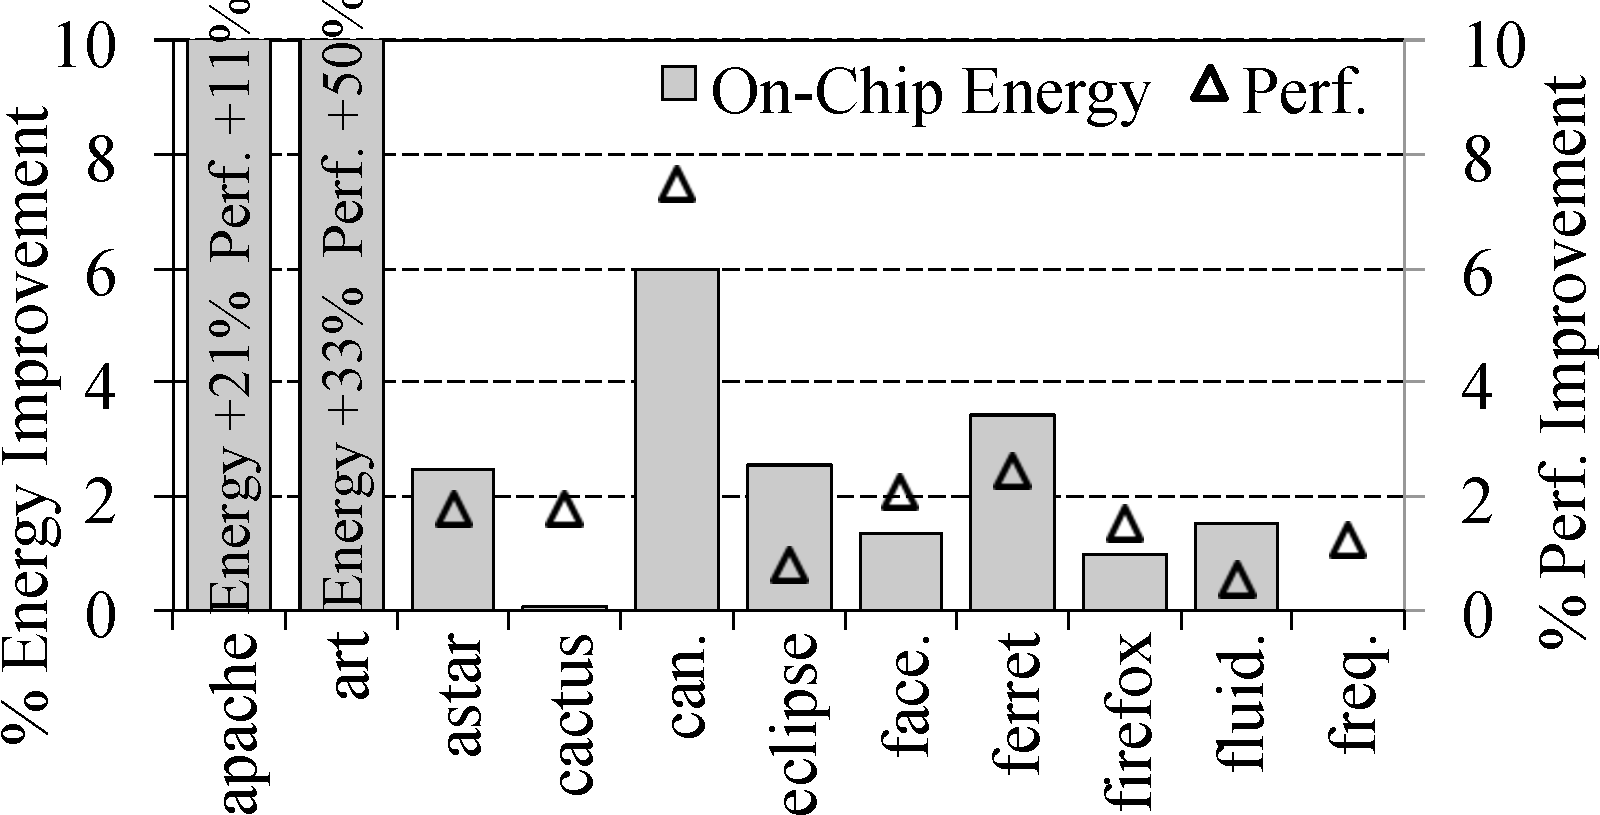
\includegraphics[width=0.7\textwidth]{files/Plots/08-DualY_Perf_Energy_A.pdf}
    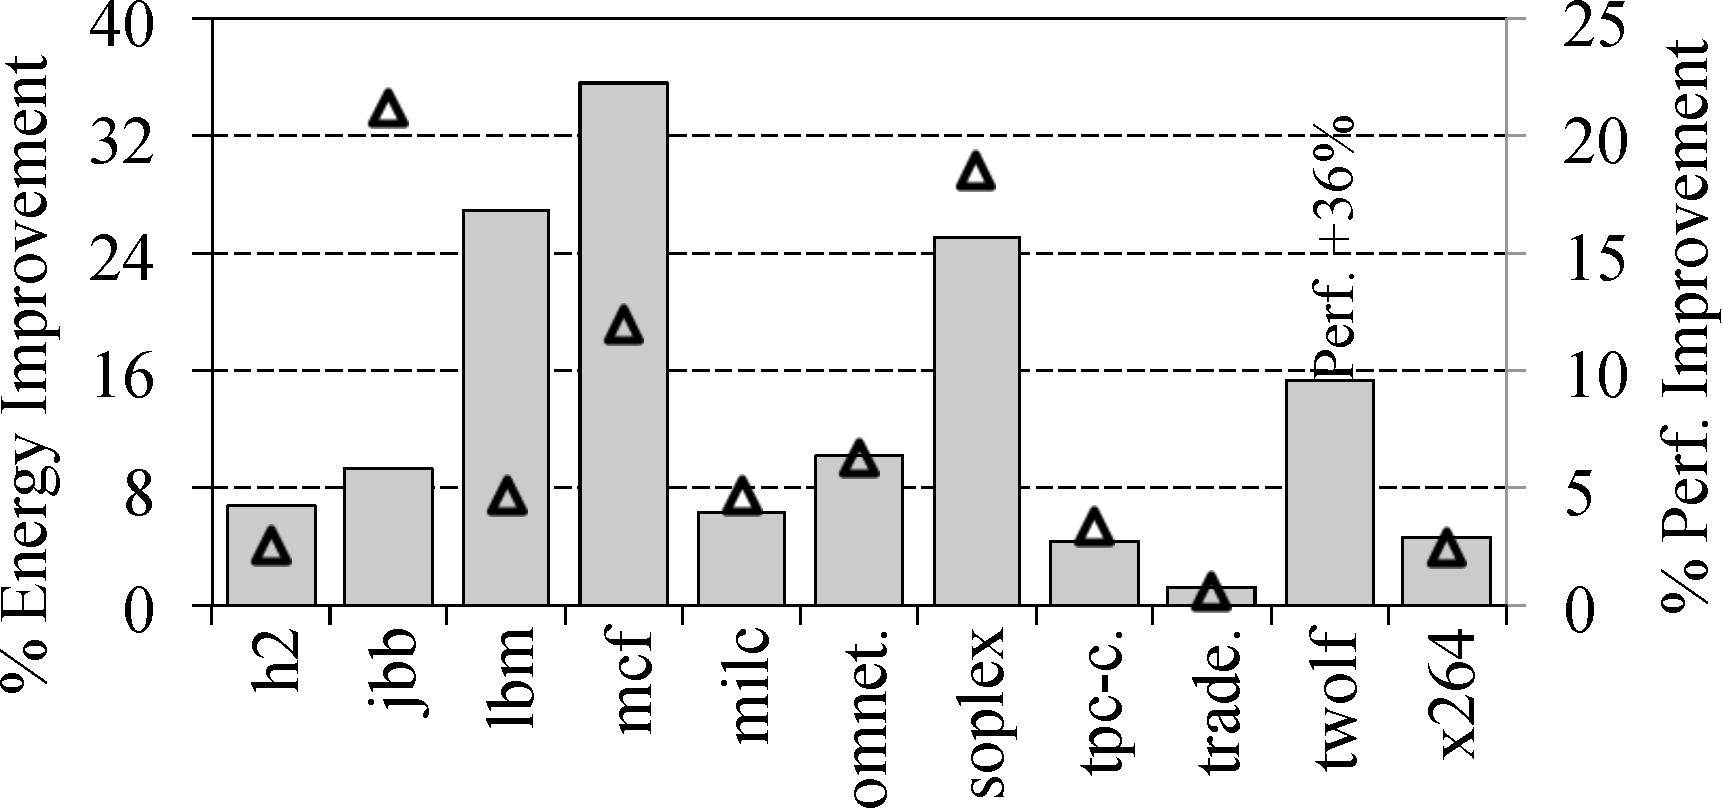
\includegraphics[width=0.7\textwidth]{files/Plots/08-DualY_Perf_Energy_B.pdf}
    \caption{Make this one chart \% improvement in performance and \% reduction in on-chip memory hierarchy energy. \\ Higher is better. Y-axis terminated to illustrate bars clearly.  Baseline: Fixed, 64K L1, 1M L2.}
    \label{plot:multi_sys_perf_energy}
\end{figure}


\section{\AC\ Adaptivity}
\label{sec:adaptivity}